\documentclass[../resumosLPOO.tex]{subfiles}

\newenvironment{conditions}
  {\par\vspace{\abovedisplayskip}\noindent\begin{tabular}{>{$}l<{$} @{${}={}$} l}}
  {\end{tabular}\par\vspace{\belowdisplayskip}}

\begin{document} 

Guarda as diferentes versões de um ficheiro como snapshots. Se não forem alterados, guarda um link para o snapshot anterior.

\paragraph{}

Tudo no git é guardado como um SHA-1.

\paragraph{}

Cada versão (commit) tem um snapshot da versão dos ficheiros (ou links caso não haja alterações). Todos os objetos (ficheiros, commits...) têm uma hash identificadora.

\paragraph{}

\begin{figure}[!h]
    \centering
    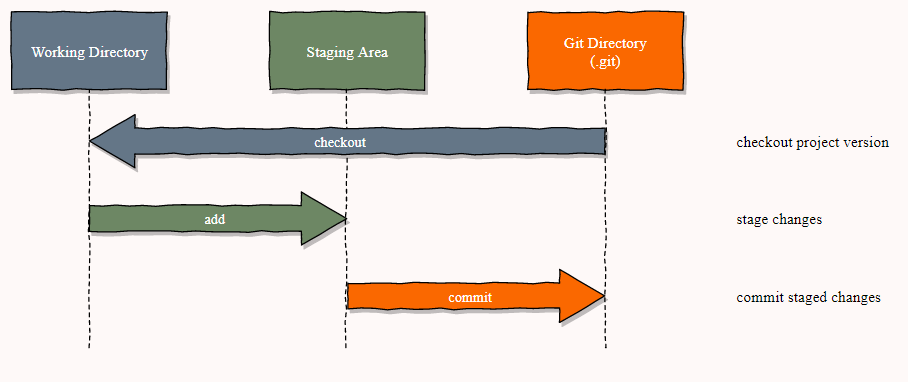
\includegraphics[width=12.5cm]{images/gitAreas.PNG}
    \caption{Git Areas}
    \label{fig:gitAreas}
\end{figure}

\paragraph{}

\begin{figure}[!h]
    \centering
    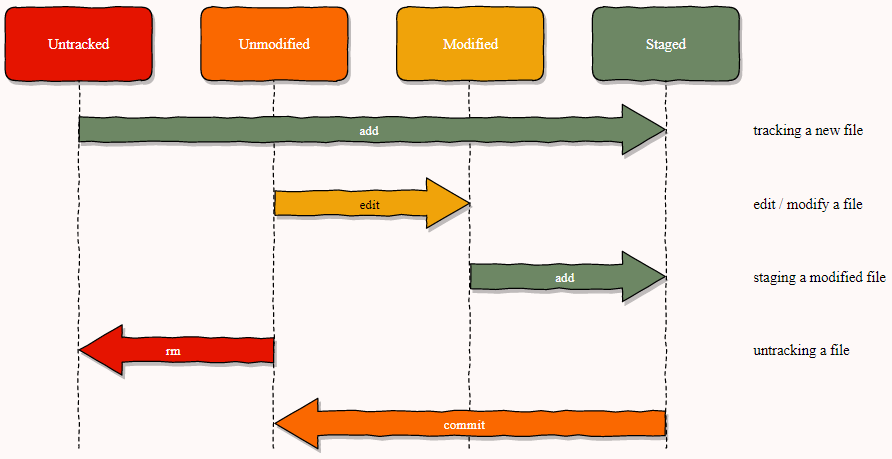
\includegraphics[width=12.5cm]{images/filesStates.PNG}
    \caption{Estados dos Ficheiros}
    \label{fig:fileStates}
\end{figure}

\paragraph{}

\lstinline{git init}: cria um subdiretório .git/ escondido

\paragraph{}

\lstinline{git add ...}
\begin{itemize}
    \item Dá track e stage a um ficheiro untracked pelo Git
    \item Dá stage a um ficheiro que foi modificado
\end{itemize}

\paragraph{}

\lstinline{git commit}: grava um novo snapshot do repositório

\paragraph{}

\lstinline{git status}: mostra o estado dos ficheiros

\paragraph{}

\lstinline{git log}: mostra o histórico de commits do repositório

\paragraph{}

Um branch é um apontador para um commit. O branch inicial é o master. 
HEAD é um apontador especial que aponta sempre para o branch atual.

\paragraph{}

\lstinline{git branch test}: cria um branch chamado \emph{test}

\paragraph{}

\lstinline{git branch}: mostra os branches atuais

\paragraph{}

\lstinline{git checkout test}: alternar para o branch \emph{test}

\paragraph{}

\lstinline{git merge test}: junta ao branch atual as modificações feitas no branch \emph{test}

\paragraph{}

Existem duas estratégias de merge:
\begin{itemize}
    \item Fast-forward merge
    \begin{itemize}
        \item Quando não existe trabalho divergente
        \item Move-se o apontador para a frente
    \end{itemize}
    \item Three-way merge
    \begin{itemize}
        \item Quando existe trabalho divergente
        \item Utiliza-se os snapshots dos dois branches e o antepassado comum e cria-se um novo commit
    \end{itemize}
\end{itemize}

\paragraph{}

\lstinline{git branch -d test}: apaga o branch \emph{test}

\paragraph{}

Ficheiros \emph{.gitignore} especificam ficheiros untracked que o git deve ignorar.

\paragraph{}

\lstinline{git clone url}: clonar/criar repositório remoto (adiciona o origin)
\begin{itemize}
    \item \lstinline{git remote -v}: lista todos os repositórios remotos
    \item \lstinline{git remove add nome url}: adicionar outro remoto
\end{itemize}

\paragraph{}

\lstinline{git fetch}: download dos ficheiros do remoto

\paragraph{}

\lstinline{git pull}: \lstinline{git fetch} + \lstinline{git merge}

\paragraph{}

\lstinline{git push}: upload das modificações realizadas

\paragraph{}

\lstinline{git reset}: reverter modificações
\begin{itemize}
    \item \lstinline{git revert <commit_id>}: caso já tenha sido realizado um push
\end{itemize}

\paragraph{}

\lstinline{COMMIT^}: commit anterior a COMMIT

\paragraph{}

\lstinline{COMMIT~2}: refere-se a 2 commits atrás de COMMIT, ou seja, ao commit anterior a \lstinline{COMMIT^}

\end{document}

